\documentclass[a4paper]{article}
\usepackage{amsthm}
\usepackage{amssymb}
\usepackage{amsbsy}
\usepackage{amsmath}
\usepackage[
  margin=1.5cm,
  includefoot,
  footskip=30pt,
]{geometry}
\usepackage{layout}
\usepackage{graphicx}
\title{Probabilistic Graphical Models : Homework 2}
\author{Raphael Avalos\\raphael@avalos.fr}
\date{2/11/18}
\graphicspath{ {./plots/} }
\begin{document}
\maketitle
\section{Exercise 1}
\subsection{Question 1}
The implied factorization for any joint distribution $p \in \mathcal{L}(G)$ is :
$$ p(x,y,z,t) = p(x)p(y)p(z|x, y) p(t|z)$$
Lets take $X\sim\mathcal{B}(p), Y\sim\mathcal{B}(p), Z=X \mathbin{\oplus} Y, T = Z$. It is clear that $X \perp\!\!\!\perp Y$ and that $X \perp\!\!\!\perp Y \not{\mid}\;Z$ because with $X$ and $Z$ we can determine $Y$. Therefore since $Z=T$, $X \perp\!\!\!\perp Y \not{\mid}\;T$
\subsection{Question 2}
\subsubsection*{1.2.a}
We consider $Z \sim \mathcal{B}(\pi)$ with $X \perp\!\!\!\perp Y \mid \;Z$ and $X \perp\!\!\!\perp Y$. We can write $p(x,y)$ in two ways:
\begin{align*}
p(x,y) &= p(x,y\mid z=0)p(z=0) + p(x,y\mid z=)p(z=1) \\
&= p(x\mid z=0)p(y\mid z=0)p(z=0) + p(x\mid z=1)p(y\mid z=1)p(z=1)
\end{align*}
And
\begin{align*}
p(x,y) &= p(x)p(y) \\
&= [p(x \mid z=0)p(z=0) + p(x \mid z=1)p(z=1)][p(y \mid z=0)p(z=0) + p(y \mid z=1)p(z=1)]
\end{align*}
Then we take the difference between those two expressions of $p(x,y)$ and factorize by $p(z=0)p(z=1)\neq0$
\begin{align*}
0 &= p(x \mid z=0)p(y \mid z=0) - p(x \mid z=1)p(y \mid z=1) + p(x \mid z=0)p(y \mid z=1) + p(x \mid z=1)p(y \mid z=0)
\end{align*}
\subsubsection*{1.2.b}
\newpage
\section{Exercise 2}
\subsection{Question 1}
Let $G = (V,E)$ be a DAF, and $i\rightarrow j$ be a covered edge of $G$. We consider $G = (V,E^\prime)$ where $E^\prime = (E \setminus \{i \rightarrow j \}) \cup \{j \rightarrow i \}$.
\begin{align*}
p(x_j \mid x_{\pi_j^G})p(x_i \mid x_{\pi_i^G}) &= p(x_j \mid x_{\pi_i^G}, x_i)p(x_i \mid x_{\pi_i^G}) \\
&= p(x_i \mid x_{\pi_i^G}, x_j)p(x_j \mid x_{\pi_i^G}) &\textit{(Bayes)} \\
&= p(x_i \mid x_{\pi_i^{G^\prime}})p(x_j \mid x_{\pi_j^{G^\prime}})
\end{align*}
Since we haven't modified any other edges, we have proven that $\mathcal{L}(G) = \mathcal{L}(G^\prime)$
\subsection{Question 2}
Let $G=(V,E)$ a directed tree and $\tilde{G}$ the symmetrized graph (which is equal to moralized graph). The cliques of $\tilde{G}$ are by the definition of a tree the set $\mathcal{C} = \{ \pi_x \mid x \in V\} \cup V$. Now let $p \in \mathcal{L}(\tilde{G})$ and consider the $\psi$ such that $\sum_{x} \prod_{c\in \mathcal{C}} \psi_c(x_c) = 1$
\begin{align*}
p(x) &= \prod_{c \in \mathcal{C}}\psi_c(x_c) \\
&= \prod_{x \in V}\psi_{x_i}(x_i)\psi_{x_i, \pi_{x_i}}(x_i,\pi_{x_i})
\end{align*}
We can define $f(x_i,x_{\pi_{x_i}}) = \prod_{x \in V}\psi_{x_i}(x_i)\psi_{x_i, \pi_{x_i}}(x_i,\pi_{x_i})$ and therefor $p \in \mathcal{L}(G)$. So $\mathcal{L}(\tilde{G}) \subset \mathcal{L}(G)$ \\
Now let $p \in \mathcal{L}(G)$
\begin{align*}
p(x) &= \prod_{x \in V} p(x \mid x_{\pi_{x}}) \\
&= \prod_{x \in V} \frac{p(\pi_{x} \mid x)}{p(\pi_x)} p(x)
\end{align*}
We can define $\psi_{x}(x) = p(x)$ and $\psi_{\pi_x}(\pi_x) = \frac{p(\pi_{x} \mid x)}{p(\pi_x)}$ and therefor $p \in \mathcal{L}(\tilde{G})$. So $\mathcal{L}(G) \subset \mathcal{L}(\tilde{G})$ \\
Finally $\mathcal{L}(G) = \mathcal{L}(\tilde{G})$
\newpage
\section{Exercise 3}
\subsection{K-mean}
We programmed k-mean++.\\\\
\begin{tabular}{|c|c|c|c|c|c|c|c|c|c|}
\hline 
• & \multicolumn{2}{c|}{Centroid 1} & \multicolumn{2}{c|}{Centroid 2} & \multicolumn{2}{c|}{Centroid 2} & \multicolumn{2}{c|}{Centroid 4} & Distortion \\ 
\hline 
1 & 3.78809 & 4.99905 & -3.79520 & -4.24816 &  3.48330 & -2.84991 & -2.14180 & 3.97338 & 3241.28275 \\ 
\hline 
2 &  3.80280 & 5.10467 & -3.81879 & -4.27423 & 3.33557 & -2.64452 & -2.240347  & 4.12744 & 3237.77959 \\ 
\hline 
3 &  3.80280 & 5.10467 & -3.81879 & -4.27423 & 3.33557 & -2.64452 & -2.24034 & 4.12744 & 3237.77959 \\ 
\hline 
4 &  3.78809 & 4.99905 & -3.66286 & -4.11101 & 3.60401 & -2.88772 & -2.15095 & 4.04338 & 3239.87631 \\ 
\hline
5 &  3.80280 & 5.10467 & -3.81879 & -4.27423 & 3.33557 & -2.64452 & -2.24034 & 4.12744 & 3237.77959 \\ 
\hline 
\end{tabular}
\\\\
The algorithm is quite stable, in 5 runs we had 3 times the same result and the other two have a 2 and 4 increase in distortion.
\subsection{EM: Covariance proportional to identity}
By applying the method of the EM algorithm we find the following.\\
The E step consist in the update of the latent varialble $q$
\begin{align*}
q^{t+1}_{k,n} = \frac{\pi_k^t p(x_n \mid \mu_k^t, {\sigma_k^t}^2)}{\sum_{x} \pi_k^t p(x \mid \mu_k^t, {\sigma_k^t}^2)} =
\frac{\frac{\pi_k^t}{\sigma_k^t} exp(-\frac{1}{2{\sigma_k^t}^2}(x_n-\mu_k^t)^T(x_n - \mu_k^t))}{\sum_{x} \frac{\pi_k^t}{\sigma_k^t} exp(-\frac{1}{2{\sigma_k^t}^2}(x-\mu_k^t)^T(x-\mu_k^t))}
\end{align*}
The M step consist in the update of $pi, \sigma, \mu$
\begin{align*}
\pi_k^{t+1} &= \frac{\sum_n q^{t+1}_{k,n}}{N} \\
\mu_k^{t+1} &= \frac{\sum_n q^{t+1}_{k,n}x_n}{\sum_n q^{t+1}_{k,n}}\\
{\sigma_k^{t+1}}^2 &= \frac{\sum_n q^{t+1}_{k,n}(x_n-\mu_k^t)^T(x_n - \mu_k^t)}{d\sum_n q^{t+1}_{k,n}}
\end{align*}
\subsection{EM: General}
\begin{align*}
q^{t+1}_{k,n} &= \frac{\pi_k^t p(x_n \mid \mu_k^t, \Sigma_k^t)}{\sum_{x} \pi_k^t p(x \mid \mu_k^t, \Sigma_k^t)} =
\frac{\frac{\pi_k^t}{\sqrt{\mid \Sigma_k^t \mid}} exp(-\frac{1}{2}(x_n-\mu_k^t)^T {\Sigma_k^t}^{-1} (x_n - \mu_k^t))}{\sum_{x} \frac{\pi_k^t}{\sqrt{\mid \Sigma_k^t \mid}} exp(-\frac{1}{2}(x-\mu_k^t)^T{\Sigma_k^t}^{-1}(x-\mu_k^t))} \\
\Sigma_k^{t+1} &= \frac{\sum_n q^{t+1}_{k,n}(x_n-\mu_k^t)(x_n - \mu_k^t)^T}{\sum_n q^{t+1}_{k,n}}
\end{align*}
\subsection{Evaluation}
\begin{tabular}{|c|c|c|}
\hline 
Log Likelihood & Iso & General \\ 
\hline 
Train & $-2689$ & $-2345$ \\ 
\hline 
Test & $-2665$ & $-2426$ \\
\hline
[Train,Test] & $-5326= -2663 * 2$ & $-4744=-2372*2$  \\
\hline 
\end{tabular}
\\\\
First, we made sure that the test data and the train data both have the same size, and therefore the comparaison of the log likelihood makes sense.
Based on the log likelihoods we can deduce that by taking $\Sigma$ proportional to the identity we produce results that are worst compared to the general case. This is not a surprise considering that the clusters aren't spheres. The other result that we can deduce from this comparaison is that the general case seems to have overfitted way more than the iso one.
\newpage
\section{Plots}
\begin{figure}[hbtp]
\caption{K-Mean++}
\centering
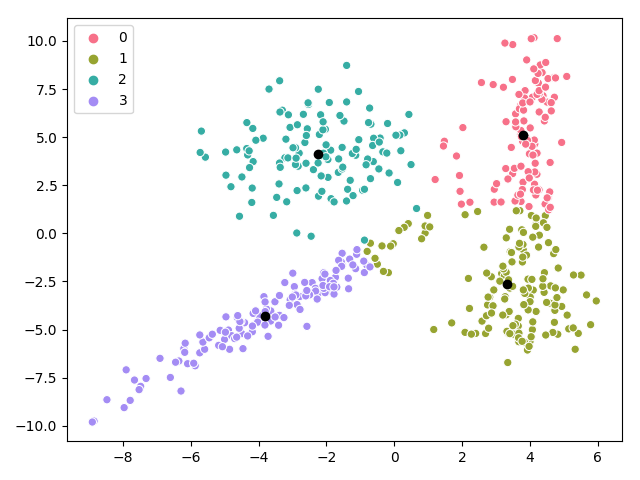
\includegraphics[scale=.4]{kmean.png}
\end{figure}

\end{document}
